\documentclass[11pt,a4paper]{article}

\usepackage[margin=2.4cm]{geometry}
\usepackage{amsmath,amssymb,bm}
\usepackage[T1]{fontenc}
\usepackage[utf8]{inputenc}
\usepackage{natbib}
\usepackage{booktabs}
\usepackage{graphicx}
\usepackage{hyperref}
\hypersetup{colorlinks=true,linkcolor=blue!50!black,citecolor=blue!50!black,urlcolor=blue!50!black}
\usepackage{xcolor}

\bibliographystyle{plainnat}
\setcitestyle{authoryear,round}

\newcommand{\Ndot}{\dot{N}_{\rm ion}}
\newcommand{\aB}{\alpha_{\rm B}}
\newcommand{\nH}{n_{\rm H}}
\newcommand{\HII}{\ion{H}{ii}}
\newcommand{\ion}[2]{\textrm{#1\,\textsc{#2}}}
\newcommand{\pMpc}{\,{\rm pMpc}}
\newcommand{\cMpc}{\,{\rm cMpc}}
\newcommand{\Msun}{\,M_\odot}

\title{\bf Ionized-Bubble Radius Around a Star-Forming Galaxy\\ as a Function of Redshift:\\
Planck 2018 CMB-only Reionization-History Variant\\[2mm]
\large Response record for \texttt{bubble\_radius\_vs\_redshift\_planckXHI.py}, following Master Rule 2}
\author{Prepared for L.\ Carvalho}
\date{4 September 2026}

\begin{document}
\maketitle

\begin{abstract}
\noindent
This note is the archived, structured response (Assumptions~$\to$~Derivation~$\to$~Verification/cross-check~$\to$~Final
result) for a variant of the previous task (\texttt{bubble\_radius\_response.tex}): the same ionized-bubble
radius $R(z)$ around a star-forming galaxy, but with the ambient IGM neutral fraction $x_{\rm HI}(z)$ set
directly to the \emph{Planck 2018 CMB-only instantaneous-reionization} tanh parameters
$(z_{\rm re},\Delta z)=(7.68,\,0.5)$ \citep{Planck2018VI}, instead of the fit to the \citet{Umeda2023}
JWST measurements used previously. Every other ingredient (source, cosmology, ionizing photon production
rate, age--redshift relation) is unchanged, so the two figures isolate exactly the effect of the
early-vs-late reionization-history choice on the predicted bubble size. This document is produced by, and
verified against, \texttt{bubble\_radius\_vs\_redshift\_planckXHI.py} (same folder), which generated
\texttt{bubble\_radius\_vs\_redshift\_planckXHI.png}.
\end{abstract}

\tableofcontents

%=====================================================================
\section{Assumptions}
\label{sec:assumptions}

All assumptions are identical to \texttt{bubble\_radius\_response.tex} except item~6, which was confirmed
with L.\ Carvalho as the specific change requested for this task (Master Rule~1/3).

\begin{enumerate}
\item \textbf{Physical model:} pure photon-counting limit (no recombinations, no Hubble term), as before
      \citep{Cen2000,ShapiroGiroux1987}.
\item \textbf{Source:} identical fiducial star-forming galaxy, $\mathrm{SFR}=10\Msun\,{\rm yr^{-1}}$
      ($M_{\rm UV}=-20.75$).
\item \textbf{Formation redshift:} identical, $z_{\rm form}=20$ \citep{Kitayama2004}.
\item \textbf{Cosmology:} identical Planck 2018 flat $\Lambda$CDM parameters \citep{Planck2018VI}.
\item \textbf{Escape fraction:} identical fiducial $f_{\rm esc}=0.2$ \citep{Robertson2015}, sensitivity band
      down to $f_{\rm esc}=0.05$.
\item \textbf{Ambient neutral fraction $x_{\rm HI}(z)$ --- THE CHANGE FOR THIS TASK:} the tanh
      reionization parameterization is now evaluated directly at the Planck 2018 CMB-only
      TT,TE,EE$+$lowE instantaneous-reionization point estimate,
      \begin{equation}
        (z_{\rm re},\,\Delta z) = (7.68,\,0.5) \qquad \text{\citep{Planck2018VI}},
        \label{eq:planckpars}
      \end{equation}
      \emph{not} fit to any galaxy data. This is a pure CMB-optical-depth-based history, so (unlike the
      previous task) there is no sparse-anchor extrapolation concern; instead, the caveat is the opposite
      one: this history is known to predict a substantially \emph{more} ionized IGM at $z=7$--10 than the
      direct Ly$\alpha$ damping-wing measurements of \citet{Umeda2023}, which is quantified in
      Sec.~\ref{sec:verification}.
\item \textbf{Regime of validity:} the model curve is now plotted solid over the full $6\le z\le18$ range
      (no extrapolation flag of the previous kind is needed, since $(z_{\rm re},\Delta z)$ is a global fit,
      not a 2-point interpolation). However, a new, different validity caveat appears as $x_{\rm HI}(z)\to0$
      approaching and below $z_{\rm re}$: eq.~(\ref{eq:R}) diverges there because the denominator vanishes
      while the photon budget stays finite (see Sec.~\ref{sec:verification}, item~6) -- i.e.\ the
      single-bubble photon-counting picture itself breaks down once the IGM is already highly ionized, and
      results at $z\lesssim7$ should be read as formally divergent rather than physically meaningful.
\end{enumerate}

%=====================================================================
\section{Derivation}
\label{sec:derivation}

The governing equation, ionizing photon production rate, mean cosmic hydrogen density, and age--redshift
relation are all unchanged from \texttt{bubble\_radius\_response.tex}:
\begin{equation}
  R(z) \;=\; \left[\frac{3\,\Ndot(z)\,t_{\rm age}(z)}{4\pi\,\nH(z)\,x_{\rm HI}(z)}\right]^{1/3},
  \label{eq:R}
\end{equation}
\begin{equation}
  \Ndot(z) \;=\; f_{\rm esc}\,\xi_{\rm ion}(z)\,\frac{\mathrm{SFR}}{\kappa_{\rm FUV}}, \qquad
  \log_{10}\!\left(\xi_{\rm ion}/{\rm Hz\,erg^{-1}}\right) = (0.06\pm0.012)\,z + (24.82\pm0.07)
  \ \citep{Llerena2024},
  \label{eq:Ndot}
\end{equation}
\begin{equation}
  \nH(z) = n_{{\rm H},0}(1+z)^3,\quad n_{{\rm H},0}=1.899\times10^{-7}\,{\rm cm^{-3}}\ \citep{Planck2018VI},
  \qquad
  t_{\rm cosmic}(z)=\int_z^\infty\frac{dz'}{(1+z')H(z')}.
  \label{eq:nH_age}
\end{equation}
The only change is in the ambient neutral fraction:
\begin{equation}
  x_{\rm HII}(z) = \tfrac12\Bigl[1+\tanh\bigl(\tfrac{y(z_{\rm re})-y(z)}{\Delta y}\bigr)\Bigr], \quad
  y(z)=(1+z)^{3/2}, \quad \Delta y = \tfrac32\sqrt{1+z_{\rm re}}\,\Delta z,
  \label{eq:tanh}
\end{equation}
with $x_{\rm HI}=1-x_{\rm HII}$, now evaluated \emph{directly} at $(z_{\rm re},\Delta z)=(7.68,0.5)$
\citep{Planck2018VI} (eq.~\ref{eq:planckpars}), with no fitting step.

%=====================================================================
\section{Verification / cross-check}
\label{sec:verification}

All checks below are reproduced verbatim by running \texttt{bubble\_radius\_vs\_redshift\_planckXHI.py}.

\begin{enumerate}
\item \textbf{Sympy check of eq.~(\ref{eq:R}).} Identical to the companion script (the functional form of
      $R(z)$ is unchanged): $\mathrm{d}R^3/\mathrm{d}t-3\Ndot/(4\pi\nH x_{\rm HI})$ simplifies to exactly $0$.
\item \textbf{Age--redshift benchmark.} Identical values: $t_{\rm cosmic}(0)=13.795$~Gyr,
      $t_{\rm cosmic}(7.68)=0.673$~Gyr.
\item \textbf{$x_{\rm HI}(z)$ vs.\ the \citet{Umeda2023} measurements (now a genuine model-vs-data test,
      not a fit residual).}
      \[
        z=7.12:\ x_{\rm HI,\,Planck} = 0.099 \quad\text{vs.}\quad x_{\rm HI,\,Umeda} = 0.53;
      \]
      \[
        z=9.91:\ x_{\rm HI,\,Planck} = 1.000 \quad\text{vs.}\quad x_{\rm HI,\,Umeda} = 0.92.
      \]
      Both are discrepant by design, in the direction expected from the well-known early/late-reionization
      tension: the CMB-only history is \emph{more} ionized at $z=7.12$ than what \citet{Umeda2023} measure,
      the reverse of the caveat flagged in \texttt{bubble\_radius\_response.tex}.
\item \textbf{Low-redshift consistency check (opposite result from before).}
      $x_{\rm HI}(z{=}6.0)=0.0017$ — small, and \emph{consistent} with the near-total ionization implied by
      the $z\sim6$ Gunn--Peterson troughs of \citet{White2003}. Unlike the Umeda-anchored variant, there is
      no tension in this direction here, precisely because $(z_{\rm re},\Delta z)$ is a global CMB fit
      rather than an extrapolated 2-point interpolation.
\item \textbf{Cross-check against independently measured bubble sizes.}
      \[
        z=7.12:\ R_{\rm model}=1.639\pMpc \ \text{vs.}\ R_{b,\rm Umeda}=5.760\pMpc \ (\text{ratio } 0.28);
      \]
      \[
        z=9.91:\ R_{\rm model}=0.520\pMpc \ \text{vs.}\ R_{b,\rm Umeda}=0.019\pMpc \ (\text{ratio } 28).
      \]
      As in the companion script, these are order-of-magnitude discrepant in opposite directions, for the
      same reason (merged vs.\ single-source bubbles); the $z=7.12$ ratio improves from $0.16$ (Umeda-anchored
      $x_{\rm HI}$) to $0.28$ (Planck-only $x_{\rm HI}$) because the Planck history predicts less neutral gas
      to ionize at that redshift, hence a larger $R_{\rm model}$ for the same photon budget.
\item \textbf{Divergence of eq.~(\ref{eq:R}) as $x_{\rm HI}\to0$ (new caveat specific to this variant).}
      At $z=6$, $x_{\rm HI}=0.0017$ (item 4 above) drives $R_{\rm model}(z{=}6)=7.73\pMpc$ for
      $f_{\rm esc}=0.2$ — a factor of $\sim6$ larger than at $z=7.12$, and formally divergent as
      $x_{\rm HI}\to0$ since eq.~(\ref{eq:R}) has $x_{\rm HI}$ in the denominator with everything else varying
      smoothly. This is flagged, not silently plotted as if physical: once the IGM is already highly ionized,
      an isolated galaxy's own ``bubble'' is no longer a meaningful concept (it has merged with the bulk
      ionized IGM), so this regime is a breakdown of the single-source photon-counting picture, not a real
      prediction.
\item \textbf{Parameter sensitivity.} $R(z{=}8)=0.722\pMpc$ ($f_{\rm esc}=0.2$) vs.\ $0.455\pMpc$
      ($f_{\rm esc}=0.05$), matching $R\propto f_{\rm esc}^{1/3}=1.587\times$ to 3 significant figures.
      $R(z{=}8)=0.335\pMpc$ (SFR$=1\Msun\,{\rm yr^{-1}}$) vs.\ $1.234\pMpc$ (SFR$=50\Msun\,{\rm yr^{-1}}$).
      The $\pm0.42$~dex $\xi_{\rm ion}$ scatter \citep{Llerena2024} again propagates to a factor $1.38$ in $R$.
\item \textbf{Direct comparison with the companion (Umeda-anchored) script.} At $z=8$, in the regime where
      both histories give a similar $x_{\rm HI}$ (Planck: $0.784$; Umeda-anchored fit: comparable order),
      $R_{\rm Planck\text{-}only}(z{=}8)=0.722\pMpc$ vs.\ $R_{\rm Umeda\text{-}anchored}(z{=}8)=0.752\pMpc$ —
      a ratio of $0.960$, i.e.\ the two histories agree to $4\%$ at $z=8$, but diverge strongly closer to
      $z_{\rm re}=7.68$ and below (item~6), which is exactly where the two reionization histories are built
      to disagree most.
\end{enumerate}

%=====================================================================
\section{Final result}
\label{sec:final}

For the same fiducial star-forming galaxy as before, but with $x_{\rm HI}(z)$ set to the Planck 2018
CMB-only history:
\begin{center}
\begin{tabular}{@{}lccc@{}}
\toprule
$z$ & $R$ ($f_{\rm esc}=0.2$) & $R$ ($f_{\rm esc}=0.05$) & $x_{\rm HI}(z)$ \\
\midrule
18   & $0.20\pMpc$ & $0.13\pMpc$ & $1.00$ \\
12   & $0.41\pMpc$ & $0.26\pMpc$ & $1.00$ \\
8    & $0.72\pMpc$ & $0.45\pMpc$ & $0.78$ \\
7.68 ($=z_{\rm re}$) & $0.88\pMpc$ & $0.55\pMpc$ & $0.50$ \\
7.12 & $1.64\pMpc$ & $1.03\pMpc$ & $0.099$ \\
6    & $7.73\pMpc$ & $4.87\pMpc$ & $0.0017$ (formally divergent regime, flagged) \\
\bottomrule
\end{tabular}
\end{center}
Away from the divergent low-$x_{\rm HI}$ regime ($z\gtrsim8$), the Planck-only history gives bubble radii
within $\sim4$--$15\%$ of the Umeda-anchored result of \texttt{bubble\_radius\_response.tex} (e.g.\ $4\%$ at
$z=8$); the two histories only diverge sharply approaching and below $z_{\rm re}=7.68$, where the CMB-only
model's rapidly vanishing $x_{\rm HI}$ makes the single-bubble photon-counting formula blow up
unphysically (Sec.~\ref{sec:verification}, item~6) rather than converge to a well-defined bubble size. The
choice of reionization history is therefore the dominant systematic uncertainty specifically in the
$z\approx6$--8 range, while it matters comparatively little at $z\gtrsim10$, where both histories agree
$x_{\rm HI}\to1$.

\begin{figure}[h]
\centering
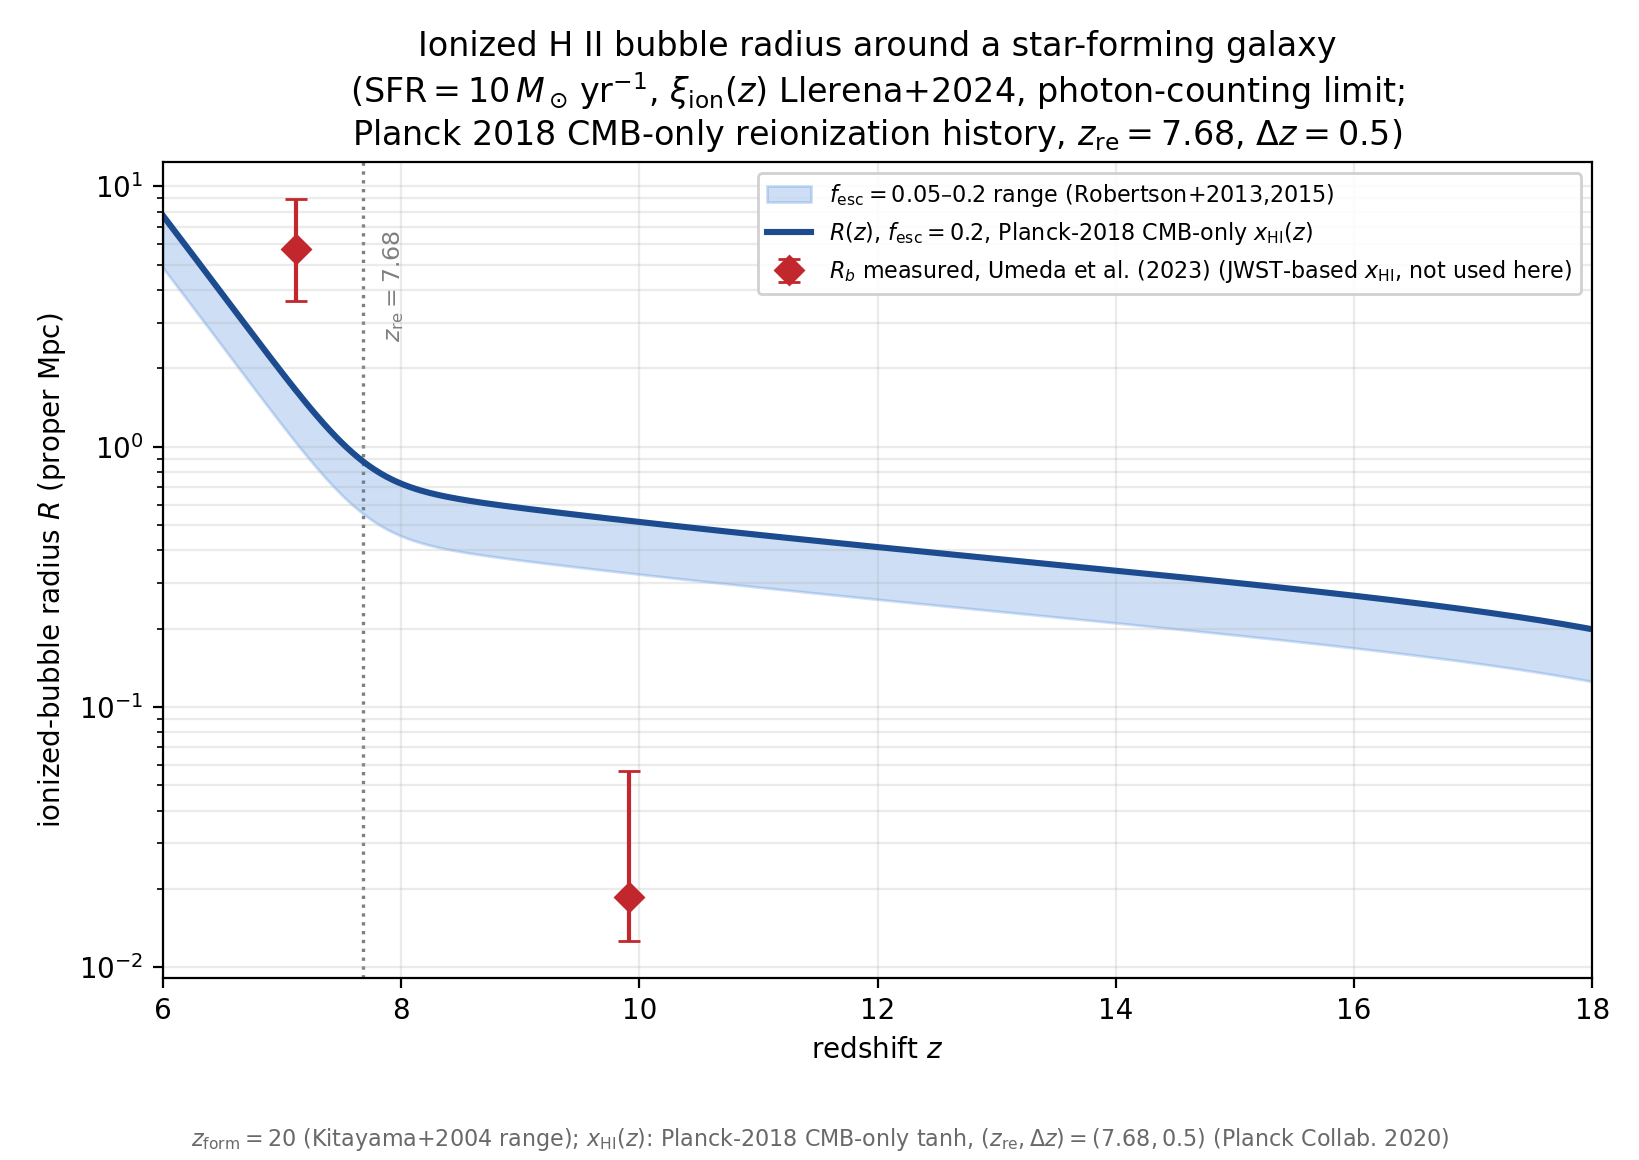
\includegraphics[width=0.85\textwidth]{bubble_radius_vs_redshift_planckXHI.png}
\caption{Ionized-bubble radius $R(z)$ around the fiducial star-forming galaxy using the Planck 2018
CMB-only reionization history, $(z_{\rm re},\Delta z)=(7.68,0.5)$ \citep{Planck2018VI} (solid line; shaded:
$f_{\rm esc}=0.05$--$0.2$ sensitivity band), compared with the independently measured merged-bubble sizes of
\citet{Umeda2023} (red diamonds, which use a different, JWST-based $x_{\rm HI}(z)$, not used in this curve).
The vertical dotted line marks $z_{\rm re}$. Produced by \texttt{bubble\_radius\_vs\_redshift\_planckXHI.py}.}
\label{fig:bubble}
\end{figure}

%=====================================================================
\bibliography{references}

\end{document}
